\documentclass[11pt,a4paper,english]{article}
    \usepackage[latin1]{inputenc}
    \usepackage{amsmath,amsfonts,amssymb}
    \usepackage{enumitem}
    \usepackage{fullpage}
    \usepackage{graphicx}
    \usepackage{tabto}
    \usepackage{etoolbox}
    \usepackage{xcolor}
    \usepackage{hyperref}
    \usepackage{minted}
    \usepackage{parskip}
    \usepackage[title]{appendix}
    \usepackage[font=small,labelfont=bf]{caption}
    \hypersetup{ colorlinks = true}
    \graphicspath{ {./} }

    \title{Bayesian Data Analysis - Assignment 8}
    \author{}

    \begin{document}
        \maketitle
      \definecolor{bg}{rgb}{0.95,0.95,0.95}
      Before digging into every model separately it would be beneficial to state about a reusable python function \textbf{show\_params} that we can use to get \textit{PSIS-LOO}, \textit{p\_eff} and to visualization \textit{k-values}.

      \begin{minted}[bgcolor=bg,linenos,fontsize=\small,autogobble]{python}
        def show_params(log_lik, fig_name, model_name):
          _psis = psis.psisloo(log_lik)
          pssloo = _psis[0]

          S = np.size(log_lik, 0)
          lppd = sum(np.log([1/S*sum(np.exp(col)) for col in log_lik.T]))
          p_loocv = lppd - _psis[0]

          hist_psis = _psis[2]

          print('PSS-LOO: ', pssloo)
          print('p_loocv: ', p_loocv)
          plt.hist(hist_psis, bins= np.linspace(0, 1, 11), ec='white')
          plt.title('k of PSIS-LOO with {0} model'.format(model_name))
          plt.savefig('./report/{0}'.format(fig_name))
          plt.figure(0)
      \end{minted}

      The above function takes \textit{log\_lik}, \textit{fig\_name} and \textit{model\_name} as parameters and prints needed values, in addition to drawing histogram. We can reuse it for every model.

      \section{Pooled model}
        In the pooled model all the machines are considered as one entity, thus we have to combine the all the measurements into one and perform our prediction on the whole data; rather than a subset. The stan model for this is stated in the \textit{Appendix A Source code}.

        We can now use our reusable function as:
        \begin{minted}[bgcolor=bg,fontsize=\small,autogobble]{python}
          fit_pooled = model_pooled.sampling(data=data_pooled)
          log_lik_pooled = fit_pooled.extract(permuted=True)['log_lik']
          show_params(log_lik_pooled, 'pooled_hist.png', 'Pool')
        \end{minted}

        \begin{itemize}
          \item \textbf{PSIS-LOO}: -130.9813139424638
          \item \textbf{p\_eff}: 2.025720004318913
          \item \textbf{k-values visualization}:
            \begin{center}
              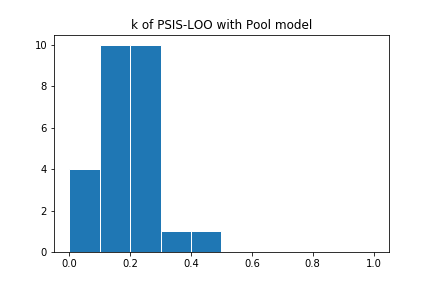
\includegraphics[width=10cm]{pooled_hist.png}
            \end{center}
          \item Stan Output:
            \begin{minted}[bgcolor=bg,fontsize=\small,autogobble]{text}
                            mean se_mean     sd   2.5%    25%    50%    75%  97.5% n_eff Rhat
              mu            93.0    0.07   3.46  86.21  90.69  93.01  95.25  99.64  2821  1.0
              sigma        18.81    0.05   2.67  14.54  16.91  18.49  20.29  24.97  2469  1.0
              ypred6       92.89    0.31  19.47  54.35  79.96  92.75 105.83 131.81  4020  1.0
              log_lik[1]   -4.01  2.9e-3   0.14  -4.31   -4.1   -4.0  -3.91  -3.75  2425  1.0
              log_lik[2]   -4.72  4.5e-3   0.26  -5.29  -4.89  -4.69  -4.54   -4.3  3257  1.0
              log_lik[3]   -3.96  2.6e-3   0.14  -4.25  -4.04  -3.95  -3.86   -3.7  2797  1.0
              log_lik[4]   -4.08  2.6e-3   0.15  -4.39  -4.17  -4.07  -3.98  -3.81  3036  1.0
              log_lik[5]   -4.15  3.0e-3   0.16  -4.48  -4.25  -4.14  -4.04  -3.88  2658  1.0
              log_lik[6]    -5.8  9.1e-3   0.52   -7.0  -6.09  -5.73  -5.43  -4.95  3299  1.0
              log_lik[7]   -3.86  2.9e-3   0.14  -4.15  -3.95  -3.85  -3.76  -3.61  2390  1.0
              log_lik[8]   -4.24  2.9e-3   0.16  -4.59  -4.35  -4.23  -4.13  -3.95  3259  1.0
              log_lik[9]   -3.86  2.8e-3   0.14  -4.15  -3.95  -3.85  -3.76  -3.61  2416  1.0
              log_lik[10]  -4.87  5.2e-3   0.29  -5.51  -5.06  -4.84  -4.66   -4.4  3178  1.0
              log_lik[11]  -3.88  2.7e-3   0.14  -4.18  -3.97  -3.88  -3.79  -3.63  2565  1.0
              log_lik[12]  -3.86  2.9e-3   0.14  -4.15  -3.95  -3.85  -3.76  -3.61  2390  1.0
              log_lik[13]  -3.86  2.9e-3   0.14  -4.15  -3.95  -3.85  -3.76  -3.61  2390  1.0
              log_lik[14]  -4.52  3.7e-3   0.22  -4.99  -4.65   -4.5  -4.37  -4.16  3335  1.0
              log_lik[15]  -3.86  2.9e-3   0.14  -4.15  -3.95  -3.85  -3.76  -3.61  2390  1.0
              log_lik[16]  -4.65  4.2e-3   0.24  -5.19   -4.8  -4.62  -4.48  -4.25  3291  1.0
              log_lik[17]  -4.01  2.6e-3   0.14  -4.31   -4.1  -4.01  -3.92  -3.75  2910  1.0
              log_lik[18]  -4.04  2.6e-3   0.14  -4.34  -4.13  -4.04  -3.94  -3.78  2973  1.0
              log_lik[19]  -7.16    0.02   0.88  -9.16  -7.68  -7.06  -6.54   -5.7  3237  1.0
              log_lik[20]  -4.04  2.6e-3   0.14  -4.34  -4.13  -4.04  -3.94  -3.78  2973  1.0
              log_lik[21]  -3.93  2.9e-3   0.14  -4.23  -4.02  -3.93  -3.84  -3.68  2349  1.0
              log_lik[22]  -3.98  2.6e-3   0.14  -4.28  -4.07  -3.98  -3.89  -3.73  2851  1.0
              log_lik[23]  -4.15  3.0e-3   0.16  -4.48  -4.25  -4.14  -4.04  -3.88  2658  1.0
              log_lik[24]  -4.24  3.2e-3   0.17   -4.6  -4.35  -4.23  -4.12  -3.95  2819  1.0
              log_lik[25]  -4.87  5.1e-3    0.3  -5.57  -5.04  -4.83  -4.66   -4.4  3294  1.0
              log_lik[26]  -3.91  2.9e-3   0.14  -4.21   -4.0  -3.91  -3.82  -3.66  2341  1.0
              log_lik[27]  -4.87  5.1e-3    0.3  -5.57  -5.04  -4.83  -4.66   -4.4  3294  1.0
              log_lik[28]  -4.65  4.2e-3   0.24  -5.19   -4.8  -4.62  -4.48  -4.25  3291  1.0
              log_lik[29]  -3.86  2.9e-3   0.14  -4.15  -3.95  -3.85  -3.76  -3.61  2390  1.0
              log_lik[30]  -3.93  2.6e-3   0.14  -4.22  -4.02  -3.93  -3.84  -3.68  2735  1.0
              lp__        -99.36    0.03   1.09 -102.1 -99.73 -99.02 -98.63 -98.35  1328  1.0
            \end{minted}
        \end{itemize}

      \section{Separate model}
        In the separate model we treat every machine as an individual entity, thus when calculating $\sigma$ or $\mu$ we take into consideration only a single machine. The combination of all machines should not effect $\sigma$ or $\mu$. The stan model for this is stated in the \textit{Appendix A Source code}.

        Again by using the reusable function we can get the quick output:
        \begin{minted}[bgcolor=bg,fontsize=\small,autogobble]{python}
          fit_separate = model_seperate.sampling(data=data_separate, n_jobs=-1)
          log_lik_separate = fit_separate.extract(permuted=True)['log_lik']
          show_params(log_lik_separate, 'separate_hist.png', 'Separate')
        \end{minted}

        \begin{itemize}
         \item \textbf{PSIS-LOO}: -132.00764178437277
         \item \textbf{p\_eff}: 9.4675135200457
          \item \textbf{k-values visualization}:
            \begin{center}
              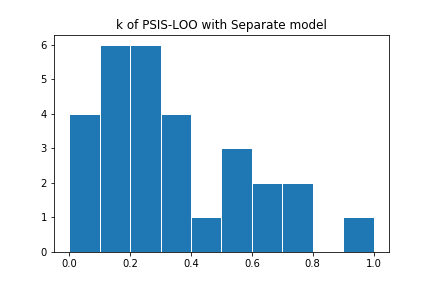
\includegraphics[width=10cm]{separate_hist.png}
            \end{center}
          \item Stan Output:
            \begin{minted}[bgcolor=bg,fontsize=\small,autogobble]{text}
                            mean se_mean     sd   2.5%    25%    50%    75%  97.5% n_eff Rhat
              mu[1]         76.3    0.42  16.62  46.74   68.5  76.22  83.83 107.37  1548  1.0
              mu[2]       106.55    0.33  10.19  86.18 101.72 106.36 110.91 127.36   956  1.0
              mu[3]        88.48    0.38   10.5  69.89  83.42  88.11  92.83 112.53   770  1.0
              mu[4]       111.93    0.18   6.37 100.45  108.9 111.73 114.76 125.41  1190  1.0
              mu[5]        90.44    0.18   7.68  75.43  86.16  90.11  94.26 107.21  1838  1.0
              mu[6]        86.06    0.38  15.27  56.09  77.97  86.13  93.54 119.75  1605  1.0
              sigma[1]     30.85    0.58  20.53  13.12  19.37  25.27  34.89  87.17  1270  1.0
              sigma[2]     18.62    0.34   11.6   7.78  11.63  15.33  21.58   50.1  1179  1.0
              sigma[3]     20.23    0.46  13.62   8.33  12.48  16.17  22.76  58.54   887  1.0
              sigma[4]     12.27    0.28   8.99   4.82   7.42   9.88  14.01  34.74  1064  1.0
              sigma[5]      16.8    0.23  10.34   6.91  10.58  14.06  19.66  43.79  2037  1.0
              sigma[6]     30.87    0.58  20.88  12.49  18.95  25.35  35.81  83.43  1308  1.0
              ypred6       85.74    0.64  38.64   7.45  65.94  85.44 105.01 161.76  3674  1.0
              log_lik[1]   -4.36    0.01   0.48  -5.49  -4.63   -4.3  -4.02  -3.62  1423  1.0
              log_lik[2]   -4.57    0.01   0.48  -5.66  -4.82  -4.51  -4.23  -3.83  1648  1.0
              log_lik[3]   -4.57    0.01   0.48  -5.66  -4.82  -4.51  -4.23  -3.83  1648  1.0
              log_lik[4]   -5.18    0.01   0.69  -6.96  -5.49  -5.05   -4.7  -4.25  4175  1.0
              log_lik[5]   -4.39    0.01   0.48  -5.51  -4.66  -4.33  -4.05  -3.63  1428  1.0
              log_lik[6]   -4.13    0.01   0.48  -5.26   -4.4  -4.06  -3.79  -3.37  1804  1.0
              log_lik[7]   -3.84    0.01   0.49  -4.99  -4.12  -3.77  -3.49  -3.06  1294  1.0
              log_lik[8]   -3.98    0.01   0.47  -5.11  -4.25  -3.92  -3.64  -3.22  1457  1.0
              log_lik[9]   -3.83    0.01    0.5  -4.99  -4.12  -3.76  -3.47  -3.05  1272  1.0
              log_lik[10]  -4.81    0.01   0.79  -6.88  -5.14  -4.63  -4.27   -3.8  3872  1.0
              log_lik[11]  -4.28    0.01    0.5  -5.46  -4.56  -4.21  -3.93  -3.53  1835  1.0
              log_lik[12]  -3.94    0.02   0.49  -5.14   -4.2  -3.87  -3.59  -3.19  1022  1.0
              log_lik[13]  -3.92    0.02    0.5  -5.13  -4.18  -3.85  -3.57  -3.16  1002  1.0
              log_lik[14]  -3.89    0.02   0.51  -5.17  -4.16   -3.8  -3.54  -3.11   955  1.0
              log_lik[15]  -4.91    0.01    0.8  -6.93  -5.24  -4.73  -4.38  -3.87  4189  1.0
              log_lik[16]  -3.67    0.01    0.5  -4.82  -3.95  -3.61  -3.31  -2.89  1191  1.0
              log_lik[17]  -3.73    0.01    0.5  -4.92   -4.0  -3.66  -3.39  -2.96  1851  1.0
              log_lik[18]   -3.5    0.01   0.49  -4.67  -3.78  -3.45  -3.16  -2.72  1309  1.0
              log_lik[19]  -3.99    0.01   0.59  -5.44  -4.28   -3.9   -3.6  -3.12  2100  1.0
              log_lik[20]   -3.5    0.01   0.49  -4.67  -3.78  -3.45  -3.16  -2.72  1309  1.0
              log_lik[21]  -4.11  9.4e-3   0.48  -5.23  -4.39  -4.05  -3.76  -3.34  2654  1.0
              log_lik[22]  -3.87    0.01   0.45  -4.87  -4.15  -3.83  -3.55  -3.13  1942  1.0
              log_lik[23]  -4.26  9.3e-3   0.55  -5.55  -4.53  -4.18  -3.89  -3.45  3464  1.0
              log_lik[24]  -4.11  9.4e-3   0.48  -5.23  -4.39  -4.05  -3.76  -3.34  2654  1.0
              log_lik[25]  -3.72    0.01   0.47  -4.76  -4.02  -3.68  -3.37  -2.94  1797  1.0
              log_lik[26]  -5.15 10.0e-3   0.71  -6.96  -5.45  -5.01  -4.69   -4.2  5060  1.0
              log_lik[27]  -4.35    0.01   0.49  -5.48  -4.65  -4.29   -4.0  -3.56  1417  1.0
              log_lik[28]  -4.64    0.01   0.48  -5.75  -4.92  -4.58  -4.29  -3.87  1973  1.0
              log_lik[29]  -4.39    0.01   0.48  -5.51  -4.68  -4.33  -4.04  -3.62  1452  1.0
              log_lik[30]  -4.51    0.01   0.47  -5.59  -4.79  -4.45  -4.17  -3.75  1627  1.0
              lp__        -81.25    0.11   3.11 -88.32 -83.19  -80.8 -78.96 -76.35   767  1.0
            \end{minted}
        \end{itemize}

      \section{Hierarchical model}
          The hierarchical model is quite interesting. It does treat every machine as a separate entity, but also computes the combination of all the machines as one entity. For that reason it can predict measurements for the machines which have no data. For example, there is no data about the seventh machine, but this model can predict its posterior distribution. The stan model for this is stated in the \textit{Appendix A Source code}.

          The same logic applies here:
          \begin{minted}[bgcolor=bg,fontsize=\small,autogobble]{python}
            fit_hierarchical = model_hierarchical.sampling(data=data_hierarchical, n_jobs=-1)
            log_lik_hierarchical = fit_hierarchical.extract(permuted=True)['log_lik']
            show_params(log_lik_hierarchical, 'hierarchical_hist.png', 'hierarchical')
          \end{minted}

        \begin{itemize}
          \item \textbf{PSIS-LOO}: -126.7561064173494
          \item \textbf{p\_eff}: 5.701680727861486
          \item \textbf{k-values visualization}:
            \begin{center}
              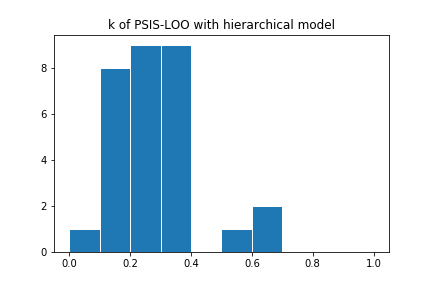
\includegraphics[width=10cm]{hierarchical_hist.png}
            \end{center}
          \item Stan Output:
            \begin{minted}[bgcolor=bg,fontsize=\small,autogobble]{text}
                            mean se_mean     sd   2.5%    25%    50%    75%  97.5% n_eff Rhat
              mu0          93.17    0.19   8.01  76.78  88.49  93.24  97.89 109.74  1790  1.0
              sigma0       16.88    0.23   9.42   5.75  10.88  14.65  20.53   40.8  1747  1.0
              mu[1]        79.64    0.14   6.76  66.08  75.27  79.47  84.13  93.32  2478  1.0
              mu[2]       103.57    0.11   6.59   90.6  99.29  103.5 107.77 116.94  3469  1.0
              mu[3]        88.82     0.1   6.24  76.49  84.73  88.86  92.96 100.93  3961  1.0
              mu[4]       107.73    0.13   6.67  94.25 103.32 107.85 112.19 120.89  2567  1.0
              mu[5]        90.72    0.09   6.11   78.5  86.75  90.72  94.66 103.07  4243  1.0
              mu[6]        87.56    0.11   6.36  75.07  83.35  87.61  91.75 100.05  3620  1.0
              sigma        15.21    0.05   2.39  11.45  13.55  14.88  16.55  20.89  2494  1.0
              ypred6       87.54    0.25   16.5  54.59  76.79  87.38  98.45 120.33  4263  1.0
              mu7          93.29    0.36  21.22   46.9  82.57  93.22 104.42 137.08  3465  1.0
              log_lik[1]   -3.76  4.6e-3   0.22  -4.28  -3.87  -3.72  -3.61  -3.42  2279  1.0
              log_lik[2]    -4.1  7.1e-3   0.41  -5.18  -4.28  -4.01  -3.82  -3.57  3335  1.0
              log_lik[3]    -4.1  7.1e-3   0.41  -5.18  -4.28  -4.01  -3.82  -3.57  3335  1.0
              log_lik[4]   -6.29    0.02   1.08   -8.7  -6.91  -6.18  -5.52  -4.51  3829  1.0
              log_lik[5]   -4.07  7.8e-3    0.4  -5.03   -4.3   -4.0  -3.79  -3.52  2584  1.0
              log_lik[6]   -4.13  6.9e-3    0.4  -5.11  -4.34  -4.06  -3.84  -3.54  3465  1.0
              log_lik[7]   -3.78  4.9e-3   0.24  -4.38  -3.91  -3.74  -3.62  -3.41  2472  1.0
              log_lik[8]   -3.96  6.0e-3   0.34  -4.78  -4.14  -3.91  -3.73  -3.47  3138  1.0
              log_lik[9]   -3.72  4.4e-3    0.2  -4.18  -3.83   -3.7  -3.59  -3.39  2056  1.0
              log_lik[10]  -4.37  8.7e-3   0.53  -5.69  -4.63  -4.25  -3.99  -3.68  3730  1.0
              log_lik[11]  -4.06  5.9e-3   0.37  -5.01  -4.24  -3.99  -3.81  -3.55  3917  1.0
              log_lik[12]  -3.76  4.3e-3   0.22  -4.27  -3.87  -3.73  -3.61  -3.42  2572  1.0
              log_lik[13]  -3.74  4.2e-3   0.21  -4.21  -3.85  -3.71   -3.6  -3.41  2402  1.0
              log_lik[14]  -3.73  4.7e-3    0.2  -4.19  -3.85  -3.71  -3.59   -3.4  1877  1.0
              log_lik[15]   -4.8  9.3e-3   0.63  -6.29  -5.15   -4.7  -4.34  -3.86  4591  1.0
              log_lik[16]  -3.75  4.4e-3   0.21  -4.25  -3.85  -3.72   -3.6  -3.41  2211  1.0
              log_lik[17]   -4.0  7.6e-3   0.36  -4.88   -4.2  -3.94  -3.74  -3.49  2277  1.0
              log_lik[18]  -3.87  6.6e-3    0.3   -4.6  -4.03  -3.82  -3.66  -3.44  2070  1.0
              log_lik[19]  -3.81  4.6e-3   0.25  -4.42  -3.92  -3.76  -3.64  -3.44  2909  1.0
              log_lik[20]  -3.87  6.6e-3    0.3   -4.6  -4.03  -3.82  -3.66  -3.44  2070  1.0
              log_lik[21]  -4.03  5.7e-3   0.35  -4.89  -4.19  -3.96  -3.79  -3.53  3609  1.0
              log_lik[22]   -3.8  4.6e-3   0.24  -4.39  -3.92  -3.77  -3.64  -3.43  2837  1.0
              log_lik[23]  -4.06  5.8e-3   0.36  -4.97  -4.23   -4.0  -3.81  -3.54  3890  1.0
              log_lik[24]  -4.03  5.7e-3   0.35  -4.89  -4.19  -3.96  -3.79  -3.53  3609  1.0
              log_lik[25]  -3.71  4.2e-3   0.19  -4.16  -3.82  -3.69  -3.58   -3.4  2089  1.0
              log_lik[26]  -5.85    0.02   0.96  -7.99  -6.42  -5.74  -5.14  -4.36  4042  1.0
              log_lik[27]  -3.77  4.3e-3   0.22  -4.29  -3.88  -3.73  -3.61  -3.43  2652  1.0
              log_lik[28]  -4.35  8.4e-3   0.51   -5.6  -4.61  -4.25  -3.99  -3.68  3629  1.0
              log_lik[29]  -3.97  5.7e-3   0.33  -4.79  -4.13  -3.91  -3.73  -3.48  3467  1.0
              log_lik[30]  -4.08  6.5e-3   0.39  -5.04  -4.27   -4.0  -3.81  -3.57  3599  1.0
              lp__        -109.0    0.07   2.52 -115.0 -110.4 -108.6 -107.1 -105.3  1209  1.0
            \end{minted}
        \end{itemize}

      \section{Summary: interpretation}
        \begin{itemize}
          \item \textbf{Pooled PSIS-LOO}: -130.9813139424638
          \item \textbf{Separate PSIS-LOO}: -132.00764178437277
          \item \textbf{Hierarchical PSIS-LOO}: -126.7561064173494
          \item \textbf{Pooled p\_eff}: 2.025720004318913
          \item \textbf{Separate p\_eff}: 9.4675135200457
          \item \textbf{Hierarchical p\_eff}: 5.701680727861486
        \end{itemize}

        From the above \textit{PSIS-LOO} list we can see that both pooled and hierarchical models are
        reliable for \textit{PSIS-LOO} estimations. The reason for these relies on the way pooled and hierarchical model use the parameters. For detailed explanation please check the discription of each model stated above.
      \begin{appendices}
        \section{Source code}
        \begin{minted}[bgcolor=bg,linenos,fontsize=\small,autogobble]{python}
          #%%
          import matplotlib
          from scipy.stats import norm
          import matplotlib.pyplot as plt
          import numpy as np
          import pandas as pd
          import pystan
          import psis

          #%% The data
          machines = pd.read_fwf('./factory.txt', header=None).values
          machines_transposed = machines.T

          def show_params(log_lik, fig_name, model_name):
              _psis = psis.psisloo(log_lik)
              pssloo = _psis[0]

              S = np.size(log_lik, 0)
              lppd = sum(np.log([1/S*sum(np.exp(col)) for col in log_lik.T]))
              p_loocv = lppd - _psis[0]

              hist_psis = _psis[2]

              print('PSS-LOO: ', pssloo)
              print('p_loocv: ', p_loocv)
              plt.hist(hist_psis, bins= np.linspace(0, 1, 11), ec='white')
              plt.title('k of PSIS-LOO with {0} model'.format(model_name))
              plt.savefig('./report/{0}'.format(fig_name))
              plt.figure(0)


          #%% Pooled model
          '''
          Pooled model
          '''
          stan_code_pooled = '''
          data {
              int<lower=0> N;       // number of data points
              vector[N] y;          //
          }
          parameters {
              real mu;              // group means
              real<lower=0> sigma;  // common std
          }
          model {
              y ~ normal(mu, sigma);
          }
          generated quantities {
              real ypred6;
              vector[N] log_lik;
              ypred6 = normal_rng(mu, sigma);
              for (i in 1:N)
                  log_lik[i] = normal_lpdf(y[i] | mu, sigma);
          }
          '''

          #%% fitting data to stan model
          machines_pooled = machines.flatten()
          model_pooled = pystan.StanModel(model_code=stan_code_pooled)
          data_pooled = dict(
              N=machines_pooled.size,
              y=machines_pooled
          )

          #%% sampling
          fit_pooled = model_pooled.sampling(data=data_pooled)
          print(fit_pooled)

          #%% hist
          log_lik_pooled = fit_pooled.extract(permuted=True)['log_lik']
          show_params(log_lik_pooled, 'pooled_hist.png', 'Pool')

          #%%
          '''
          Separate model
          '''
          stan_code_separate = '''
          data {
              int<lower=0> N;               // number of data points
              int<lower=0> K;               // number of groups
              int<lower=1,upper=K> x[N];    // group indicator
              vector[N] y;
          }
          parameters {
              vector[K] mu;                 // group means
              vector<lower=0>[K] sigma;     // group stds
          }
          model {
              y ~ normal(mu[x], sigma[x]);
          }
          generated quantities {
              real ypred6;
              vector[N] log_lik;
              ypred6 = normal_rng(mu[6], sigma[6]);
              for (i in 1:N)
                  log_lik[i] = normal_lpdf(y[i] | mu[x[i]], sigma[x[i]]);
          }
          '''

          #%% fitting data into the stan model
          model_seperate = pystan.StanModel(model_code=stan_code_separate)
          data_separate = dict(
              N=machines_transposed.size,
              K=6,
              x=[
                  1, 1, 1, 1, 1,
                  2, 2, 2, 2, 2,
                  3, 3, 3, 3, 3,
                  4, 4, 4, 4, 4,
                  5, 5, 5, 5, 5,
                  6, 6, 6, 6, 6,
              ],
              y=machines_transposed.flatten()
          )

          #%% sampling
          fit_separate = model_seperate.sampling(data=data_separate, n_jobs=-1)
          print(fit_separate)

          #%% hist
          log_lik_separate = fit_separate.extract(permuted=True)['log_lik']
          show_params(log_lik_separate, 'separate_hist.png', 'Separate')

          #%%
          '''
          Hierarchical model
          '''
          stan_code_hierarchical = '''
          data {
              int<lower=0> N;             // number of data points
              int<lower=0> K;             // number of groups
              int<lower=1,upper=K> x[N];  // group indicator
              vector[N] y;
          }
          parameters {
              real mu0;                   // prior mean
              real<lower=0> sigma0;       // prior std
              vector[K] mu;               // group means
              real<lower=0> sigma;        // common std
          }
          model {
              mu ~ normal(mu0, sigma0);
              y ~ normal(mu[x], sigma);
          }
          generated quantities {
              real ypred6;
              real mu7;
              vector[N] log_lik;
              ypred6 = normal_rng(mu[6], sigma);
              mu7 = normal_rng(mu0, sigma0);
              for (i in 1:N)
                  log_lik[i] = normal_lpdf(y[i] | mu[x[i]], sigma);
          }
          '''

          #%% fitting data into the stan model
          model_hierarchical = pystan.StanModel(model_code=stan_code_hierarchical)
          data_hierarchical = dict(
              N=machines_transposed.size,
              K=6,
              x=[
                  1, 1, 1, 1, 1,
                  2, 2, 2, 2, 2,
                  3, 3, 3, 3, 3,
                  4, 4, 4, 4, 4,
                  5, 5, 5, 5, 5,
                  6, 6, 6, 6, 6,
              ],
              y=machines_transposed.flatten()
          )

          #%% sampling
          fit_hierarchical = model_hierarchical.sampling(data=data_hierarchical, n_jobs=-1)
          print(fit_hierarchical)

          #%% hist
          log_lik_hierarchical = fit_hierarchical.extract(permuted=True)['log_lik']
          show_params(log_lik_hierarchical, 'hierarchical_hist.png', 'hierarchical')
        \end{minted}
      \end{appendices}
  \end{document}
